\documentclass[14pt]{extarticle}

\usepackage{geometry}
\usepackage{amsmath,amsthm,amssymb}
\usepackage[utf8]{inputenc}
\usepackage[T1,T2A]{fontenc}
\usepackage{bold-extra}
\usepackage[english,russian]{babel}
\usepackage{indentfirst}
\usepackage{graphicx}
\graphicspath{ {images/} }
\usepackage{float}
\usepackage{listings}
\usepackage{lmodern}
\usepackage{appendix}
\usepackage{braket}
\usepackage{cite}
\usepackage[nottoc,numbib]{tocbibind}

\geometry{
a4paper,
left = 20mm,
right = 15mm,
bottom = 20mm,
top = 20mm,
}
\renewcommand{\rmdefault}{ftm} % TimesNewRoman
\renewcommand{\baselinestretch}{1.5} 

\begin{document}

\begin{titlepage}
	\begin{center}
		\small{ФЕДЕРАЛЬНОЕ ГОСУДАРСТВЕННОЕ БЮДЖЕТНОЕ ОБРАЗОВАТЕЛЬНОЕ}\\ 
			УЧРЕЖДЕНИЕ ВЫСШЕГО ОБРАЗОВАНИЯ\\
			«МОСКОВСКИЙ ГОСУДАРСТВЕННЫЙ УНИВЕРСИТЕТ\\
			имени М.В.ЛОМОНОСОВА»\\
		\hfill \break
		ФАКУЛЬТЕТ ВЫЧИСЛИТЕЛЬНОЙ МАТЕМАТИКИ И КИБЕРНЕТИКИ\\
		КАФЕДРА СУПЕРКОМПЬЮТЕРОВ И КВАНТОВОЙ ИНФОРМАТИКИ\\
		\vfill
		ЗАДАНИЕ 1 \\
		\textbf{<<АНАЛИЗ ВЛИЯНИЯ КЭША НА ОПЕРАЦИЮ МАТРИЧНОГО УМНОЖЕНИЯ>>}\\
	\end{center}	
	\vfill
	\begin{flushright}
		Выполнил студент \\
		группы м118:\\
		Пухов Д. Н.\\
		{\hspace{3cm}}
	\end{flushright}
	
	
	\begin{center}
		Москва \\
		2017 
	\end{center}
	
	\thispagestyle{empty}

\end{titlepage}





\section*{Формулировка задачи} 
Исследовать зависимость скорости простейшего алгоритма перемножения двух
плотных матриц от порядка индексов. Проверить результаты вычислений сторонней программой.

\section*{Описание алгоритма}
Уравнение $ C = A \cdot B $, где $ A = n \times m $, $ B = m \times h $, $ C = n \times h $, можно переписать следующим образом:
\begin{equation*}
c_{ij} = \sum \limits_{k=0}^{k=m-1} a_{ik} b_{kj}, \quad i = \overline{0,n-1}, \quad j = \overline{0,h-1},
\end{equation*}
что соответствует следующему коду на языке C:
\begin{lstlisting}[language=C]
for(int i=0; i<n; ++i)
	for(int j=0; j<h; ++j)
		for(int k=0; k<m; ++k)
			C[i][j] += A[i][k] * B[k][j];
\end{lstlisting}

Меняя порядок индексов, можем получить 6 алгоритмов: ijk, jik, ikj, kij, kji, jki.

\newpage

\section*{Описание программы}
\subsection*{Запуск}
Программа использует Makefile и может выполнять два задания:
\begin{itemize}
\item make test - последовательно запускается каждый из 6 алгоритмов, результаты записываются в файлы, и проверяются на корректность с помощью python и numpy;
\item make report - вычисляются средние времена работы каждого алгоритма, записываются в файл, затем строится график с использование python и matplotlib.
\end{itemize}

\subsection*{Формат запуска из командной строки}
\$ <программа> <флаг типа> <режим> (<файл матрицы A> <файл матрицы B> <файл матрицы C> | <файл для результатов>)

Пример: \$ ./calc -f 0 A.bin B.bin C.bin

Пример: \$ ./calc -f 6 times.bin

\subsection*{Формат записи в файл}
Записи осуществляются в бинарном виде.

Матрица $ n \times m $ записывается в следующем порядке:
\begin{itemize}
\item int type - 0 или 1 в соответствии с типом данных (float или double),
\item int n, int m,
\item float A[n*m] или double A[n*m], построчно.
\end{itemize}
Результаты (времена работы) записываются как массив из 6 элементов типа double.

\newpage

\section*{Результаты}
На графике показано время работы простейшего алгоритма перемножения матриц в зависимости от порядка индексов суммирования. Для объяснение результатов достаточно рассмотреть, как происходит обращение к элементам матриц в алгоритме (принимая во внимание, что матрицы хранятся построчно в виде одномерных массивов):
\begin{lstlisting}[language=C]
C[i*h+j] += A[i*n+k] * B[k*h+j];
\end{lstlisting}
Ключевой аспект --- хранение данных в кэше первого уровня. Данные загружаются в кэш кусками длиной в размер линии кэша, размер которой на моём ПК --- 64 байта. Общий объём кэша первого уровня --- 32 Кбайта, т.е. 32 * 1024 / 64 = 512 линий. Одна линия кэша вмещает либо 8 чисел с плавающей запятой двойной точности (double), либо 16 чисел с плавающей запятой одинарной точности (float).

Значит, эффективнее "бежать" последовательно по элементам строки, чем по элементам столбца (которые удалены друг от друга на расстояние длины строки). То есть внутренний цикл будет крайне медленным, если будет использовать индекс $i$: элементы матриц A, C "пробегаются" по столбцам, элемент матрицы B --- константа. Если внутренний цикл использует индекс $k$, то элемент матрицы C есть константа, элементы матрицы A достигаются построчно, матрицы B --- по столбцу. Наконец, при индексе $j$ матрицы C и B используется построчно, элемент матрицы A --- константа. Это, очевидно, наилучший сценарий.

\begin{figure}[H]
	\centering
	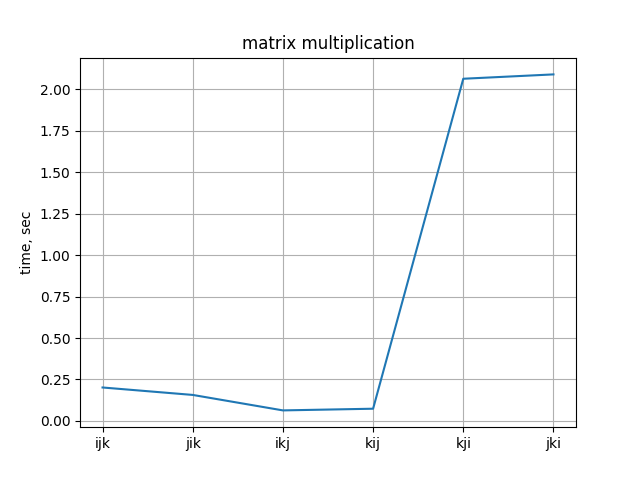
\includegraphics[scale=1]{Figure_1}
	\caption{Времена работы при различном порядке индексов}
\end{figure}

\end{document}